\documentclass[12pt]{article}
\usepackage{geometry}
\geometry{margin=1in}
\usepackage{graphicx}
\usepackage{listings}
\usepackage{hyperref}
\usepackage{parskip}
\lstset{basicstyle=\ttfamily\small,breaklines=true}
\begin{document}
\begin{titlepage}
  \centering
  \vspace*{4cm}
  {\LARGE \textbf{Security Protocols and their Formal Analysis} \par}
  \vspace{1cm}
  {\Large Case Studies and Formal Models with ProVerif and Tamarin \par}
\end{titlepage}

\begin{abstract}
This document revisits classical security protocol design and applies modern formal verification techniques to the TLS 1.3 core handshake. It compares historical protocol notation with modern symbolic and computational models, applies structured threat modeling to medical, financial, and defense case studies, and provides runnable ProVerif and Tamarin models in the appendix.
\end{abstract}

\tableofcontents
\listoffigures
\listoftables

\section{Introduction}
Security principles (confidentiality, integrity, availability, authenticity) remain central to software engineering. This assignment updates the SPR material to 2025...

\section{Secure Communication Protocols}
\begin{figure}[h]
\centering
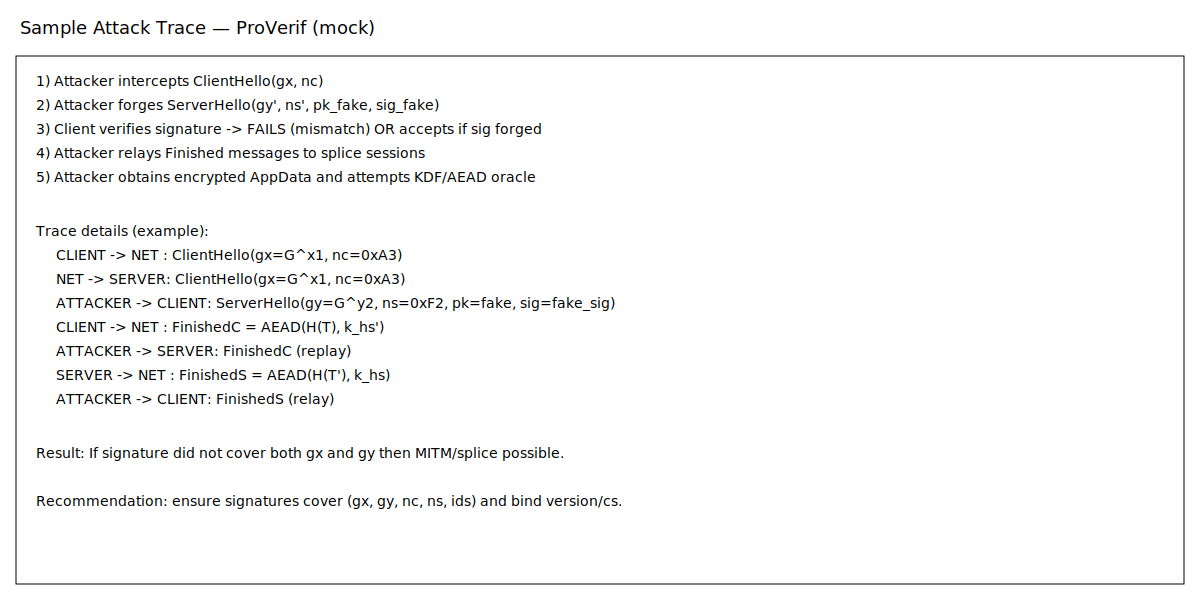
\includegraphics[width=0.6\textwidth]{sample_attack_trace.svg}
\caption{Simplified TLS 1.3 Handshake Flow (placeholder)}
\end{figure}

\subsection{Formal Snippets}
\begin{lstlisting}
equation dh(exp(g(), x), y) = dh(exp(g(), y), x).
\end{lstlisting}
\begin{lstlisting}
lemma forward_secrecy: ...
\end{lstlisting}

\section{Containment vs Publisher Trust}
Discussion...

\section{Case Studies...}
Discussion...

\section{Discussion and Future Directions}
Discussion...

\section{Conclusion}
Conclusion...

\appendix
\section{ProVerif model}
\lstinputlisting{tls13_strict.pv}

\section{Tamarin model}
\lstinputlisting{TLS13_Strict.spthy}

\end{document}